\section{Systemarchitektur}

\begin{figure} 
  \centering
     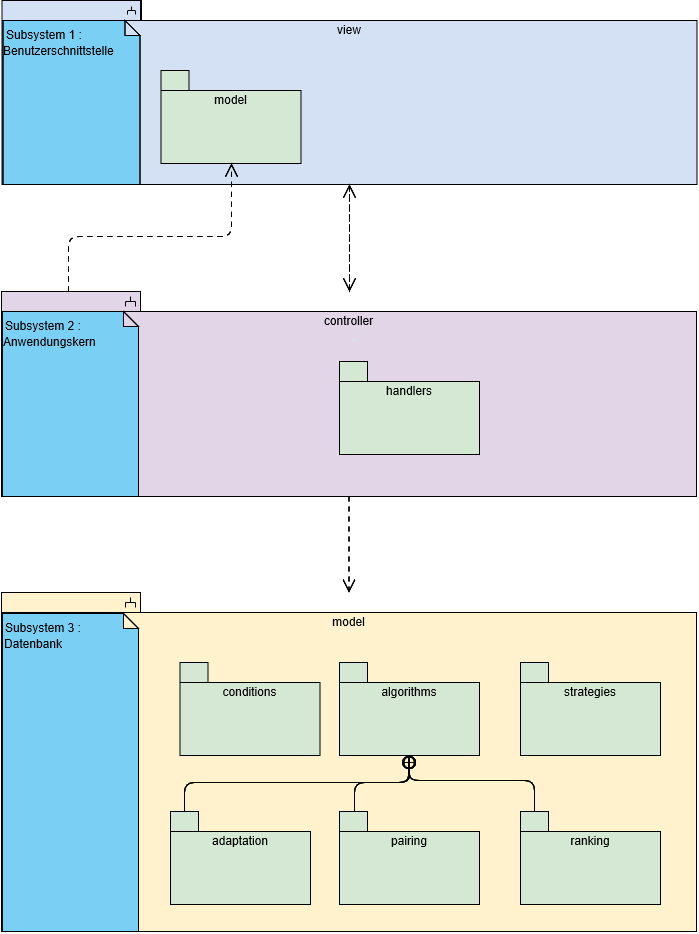
\includegraphics[width=1.1\textwidth]{Systemarchitektur/UMLzuGrobentwurf.png}
\end{figure}

SSWIS baut auf einem MVC-Model auf, welches um ein ViewModel erweitert wurde. Die Benutzerinteraktion erfolgt
über die View. Im ViewModel werden die Benutzereingaben zwischengespeichert und auf Korrrektheit überprüft. Des Weiteren schreibt der Controller die Informationen in das ViewModel, die auf der Benutzeroberfläche angezeigt werden sollen. Der Controller ist für die Programmflusssteuerung zuständig. Die ActionListener der Benutzeroberfläche sind im Controller implementiert, dadurch kann man neue Benutzeroberflächen erstellen und die ActionListener wieder verwenden. Außerdem dient der Controller zum Kommunikation zwischen View und Model .Im Model sind die Objekte der Simulation abgebildet, dort ist die gesamte Business Logic implementiert.
